\documentclass{article}
\usepackage{graphicx}
\usepackage{amsfonts}
\usepackage{amsmath}
\usepackage{braket}
\usepackage{tikz}
\usepackage{float}
\usetikzlibrary{quantikz2}
\usepackage{pgfplots}
\pgfplotsset{compat=1.18}
\title{Quantum Error Correction Tecniques}
\author{Alessio Delli Colli}
\date{May 2024}

\newtheorem{theorem}{Theorem}

\begin{document}

\maketitle

\newpage

\tableofcontents

\newpage

\section{Introduction}

\vspace{10pt}

\subsection{The importance of quantum information}

\vspace{10pt}

Maintaining fundamental properties of important documents, like secrecy
and authenticity, through the process of digitalization has been one of the main
quests of the last decades. These qualities have been currently achieved mainly
by the route of clever mathematics, exploiting properties of our current com-
puting machines and especially the knowledge, although not yet crystal clear,
of what they can or can’t do in a reasonable time.
It is possible to find a relevant example of this in the RSA protocol, that uses
the difficulty of solving the factorization problem in available machines in order
to construct a cryptosystem and also a digital signature scheme wow.

\vspace{10pt}

\noindent While the metric of ”being difficult to compute” may seem arbitrary at first
glance, it is based on the solid theory of computational complexity.
Such theory, founded on the Church-Turing Thesis, aims to measure the com-
plexity of a problem in terms of the number of steps a Turing machine would
take to solve it.
More specifically, problems are said to be in the class P if there is a Turing
machine able to solve them in an amount of time that is a polynomial function
of the input size and are said to be in the class NP if there is a Turing machine
that can verify a guessed solution in a similar polynomial time.
The distinction between the classes P and NP has yet to be proved but it is
generally assumed that these classes are not coincident.

\vspace{10pt}

\noindent This conjecture leads to believe that there are some problems that belong to
the class NP but not to P so, for them, it is easy to verify if a configuration is
a solution but not to find one. For these problems isn’t thus possible to find a
solving algorithm that is substantially better than trying all the possible config-
urations and verifying them one by one until a solution is found. This approach
is known as an exhaustive search.
If we were able to test the configurations efficiently that would lead to the possi-
bility of constructing an algorithm that solves a problem without the knowledge
of its structure, but just utilizing an ”oracle” which is a routine that is able to
distinguish solutions from non solutions.
Such approach is called a Black-Box algorithm.
Unfortunately it is known that classical computation can’t make this kind of al-
gorithm efficient but maybe in another form of computation the outcome could
be different.

\newpage

\noindent In 1996 Lov Grover showed that with quantum computing it is possible to
complete an exhaustive search with only square root of n calls to the oracle,
where n is the size of the input. While this is an extraordinary result, later
studies have shown that it can’t be further improved.
This means that no Black-Box algorithm can solve a non polynomial problem
in polynomial time, even taking into consideration quantum computing.
Though, quantum computing can be much more significative when the algorithm
relies on the problem structure, as in the case of Shor’s algorithm.
The Shor’s algorithm aims to find a solution to the factorization problem by
doing a reduction to a simpler problem, at least from a quantum standpoint,
which is finding the order of an element in an abelian group. This problem is
then solved thanks to a procedure called Quantum Fourier Transform.
The whole procedure has a just above quadratic time complexity and so, it is
much faster than the better classical algorithm currently available which works
is a sub-exponential time.
The execution of this algorithm or it’s proper variants on a suitable hardware
could allow to break most of the cryptosystems used today, like DHM, ECDHM,
and the above mentioned RSA.

\vspace{20pt}


\subsection{The need for quantum error correction}

\vspace{10pt}

The applications described above although feasible for quantum computers require
very complex machines that are prone to errors.
This comes from the fact that larger machines have a tendency to bond to the
environment and this bonding makes them produce unpredictable results.
Such tendency has put a limit to the implementation of quantum algorithms.
An example of that could be that the largest number we have currently been
able to reliably factorize using the Shor algorithm is 21.
This seems rather underwhelming given the fact the numbers we aim to factorize
whit it are in the realm of $2^{2000}$.
Luckly there are techniques that allow us to catch and correct the errors
when they arise, before they can propagate uncontrollaby and improving
such tecniques will bring us closer to our goal.



\section{From quantum physics to quantum information}

To understand the technicalities behind the operations described above it is
necessary to dive in the phisical processes involved in them.\\
So will be done shortly in this section.

\newpage

\subsection{Foundations of quantum mechanics}

\subsubsection{Cinematic axioms}

\begin{enumerate}
	\item To each quantum system S corresponds an Hilbert space $H_S$.\\
	      The space of pure\footnote{The definition of pure state will
		      be given in the section 4}
	      states is identified by the projective space $P(H_S)$.

	\item Given two quantum systems $S_1$ and $S_2$ and their correspondent
	      Hilbert spaces $H_{S1}$ and $H_{S2}$ the space that characterizes the
	      compound system is $H_{S1} \otimes H_{S2}$, where $\otimes$ denotes
	      the tensor product.

	\item A measure procedure on a quantum state S is described
	      by a family \\  $M := \{M_\alpha \}_{\alpha\in A}$ where:

	      \begin{itemize}
		      \item $M_\alpha \in B(H_S) $ $ \forall \alpha \in A$
		      \item $A \subset \mathbb{R}$
		      \item $\sum_{\alpha \in A} M_\alpha^\dag M_\alpha = Id(H_S)$
	      \end{itemize}

	      Where B(Hs) is the set of bounded operators in $H_S$ and A is the
	      set of all the possible outcomes of the measure.\\
	      Given the outcome $\alpha_0 \in A$ and the state $\ket{\psi}$,
	      the probability
	      of measuring the output $\alpha_0$ being in the state $\ket{\psi}$
	      is:
	      \begin{center}
		      $P(\psi : \alpha_0) = \braket{\psi|M_{\alpha_0}^\dag M_{\alpha_0}\psi}$

	      \end{center}


	      \subsubsection{Dynamic axioms}


	\item Given a quantum system $S_1$ and two time instants$ t_1$ and $t_2$
	      with $t_1<=t_2$ there is an unique unitary operator$U(t_1,t_2)$ that
	      describes the evolution of the system between the time instants.

	      The unitary operator should respect also some additional
	      properties:\\
	      $
		      \begin{cases}
			      U(t_1,t_1) = Id(H_S) \\
			      U(t_2,t_3)U(t_1,t_2) = U(t_1,t_3)
		      \end{cases} $

	\item In the instant immediately after the measure
	      $M := \{M_\alpha \}_{\alpha\in A}$ is applied to the quantum
	      system S while being in the state $\ket{\psi}$ \\
	      the system will collapse to the state:

	      \begin{center}
		      $\dfrac{M_{\alpha_0}\ket\psi}
			      {\sqrt{\braket{\psi|M_{\alpha_0}^\dag M_{\alpha_0}\psi}}}$
	      \end{center}
\end{enumerate}


\subsection{Qubits}

Physical systems can be used to store information
but not all systems are practical for doing so. \\
In fact, if we wanted to represent some complex information we
could choose to use a single complex system that has many states,
but doing so it would be very difficult to prepare it for the
computation.\\
Suppose for example that we had a way of quickly giving energy
to the system to make it jump from one of its base states to
the next, and luckily we have it.\\
In the case of one single system to reach the n-Th base state
we would need n energy transfers, and that is quite unpractical.\\
Even more so if we consider than using multiple occurrences of
the simplest non trivial quantum system, that is the one that
has only 2 base states,\\ we would need at most $\log_2{n}$ transfers.\\
This simple quantum system is known as a qubit.\\

\subsection{Qubit representations and Probability amplitudes}

The state of a qubit can be represented in many ways.\\
Some useful representations are the unitary vectors in $\mathbb{C}^2$
and the points of a unitary sphere called the Block Sphere.
we are going to analyze each of them and their respective advantages.

\subsubsection{State vectors}

The state vector of a qubit consists in two components in $\mathbb{C}$
that can be interpreted as the probability amplitudes of each of the
base states.
The probability amplitude of a base state is a complex number that,
when taken the absolute value squared, gives the probability that the
above mentioned state will be the outcome
of a measure. %FIXME rivedere la fine


\subsubsection{The Bloch sphere}

\begin{center}
	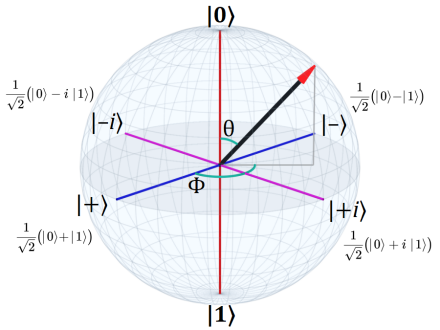
\includegraphics[scale=0.5]{bloch-sphere.png}
\end{center}
The Bloch sphere gives us an useful graphical representation of a
qubit's state that is linked to the state vector by the following
isomorphism.\\

\begin{equation}
	\ket{\psi} = \cos{\dfrac{\theta}{2}}\ket{0}+e^{i\phi}\sin{\dfrac{\theta}{2}}\ket{1} \\
\end{equation}
This representation is particularly advantagious because it allows
to visualize the evolution of a qubit over time in the execution
of a quantum algorithm.


\section{One qubit systems}


\subsection{Introduction to quantum gates}
Quantum states are not very interesting when they are static, \\
what we want to achieve is a way to make them evolve\\
and accurately control their evolution over time.
The element used in a quantum system in order to make it evolve
in a controlled way is called a quantum gate.\\
While in classical information there is just a single kind of one bit
gate in quantum information there are infinitely many!
In the next paragraph we will se the most important ones.

\newpage

\subsection{Some examples of one qubit gates}

\begin{itemize}

	\item Pauli Gates\\
	      can be seen as rotations on the three main axis of the bloch
	      sphere
	      \begin{center}
		      $	X:=\begin{bmatrix}
				      0 & 1 \\
				      1 & 0
			      \end{bmatrix}
			      \hspace{10pt}
			      Y:=\begin{bmatrix}
				      0 & -i \\
				      i & 0
			      \end{bmatrix}
			      \hspace{10pt}
			      Z:=\begin{bmatrix}
				      1 & 0  \\
				      0 & -1
			      \end{bmatrix}$
	      \end{center}


	\item Hadamard Gate\\
	      brings the state $\ket{0}$ to
	      $\ket{+} := \dfrac{\ket{0}+\ket{1}}{2}$
	      and the state $\ket{1}$ to $\ket{-} := \dfrac{\ket{0}-\ket{1}}{2}$
	      \begin{center}
		      $	H:=\dfrac{1}{\sqrt{2}}\begin{bmatrix}
				      1 & 1  \\
				      1 & -1
			      \end{bmatrix}$
	      \end{center}

	\item Phase Gates \\
	      change the phase of a qubit arbitrarly or by a fixed ammout
	      \begin{center}
		      $	P:=\begin{bmatrix}
				      1 & 0         \\
				      0 & e^{i\phi}
			      \end{bmatrix}
			      \hspace{10pt}
			      S:=\begin{bmatrix}
				      1 & 0                   \\
				      0 & e^{i\tfrac{\pi}{2}}
			      \end{bmatrix}
			      \hspace{10pt}
			      T:=\begin{bmatrix}
				      1 & 0                   \\
				      0 & e^{i\tfrac{\pi}{4}}
			      \end{bmatrix}$
	      \end{center}
\end{itemize}

\subsection{One qubit interference}




The reason why quantum algorithms can be faster than classical ones
in some tasks is because they can exploit some propreties of quantum
systems that classical systems lack. \\
One of these propreties is interference.\\
In quantum information interference is used to enhance the probability of
getting a favourable state at the end of the computation.\\
\vspace{10pt}
\begin{figure}[H]
	\centering
	\scalebox{1.5}{
		\begin{quantikz}
			\lstick{$\ket{0}$}\slice[style=blue, label style={pos=1, anchor=north}]{${\scriptstyle\ket{\psi_{t0}}}$}	& \gate{H}
			\slice[style=blue, label style={pos=1, anchor=north}]{${\scriptstyle\ket{\psi_{t1}}}$}	& \gate{P}
			\slice[style=blue, label style={pos=1, anchor=north}]{${\scriptstyle\ket{\psi_{t2}}}$}	& \gate{H}
			\slice[style=blue, label style={pos=1, anchor=north}]{${\scriptstyle\ket{\psi_{t3}}}$}	&
		\end{quantikz}
	}
	\caption{Ramsey interferometer}
	\label{interference}
\end{figure}
\vspace{10pt}
\noindent An example of this can be found in the circuit in Figure \ref{interference}.\\
The circuit, called Ramsey interferometer, can be modeled by two Hadamard gates with a phase gate
in between.\\
\newpage
\noindent Below is the time analisys of the circuit.
\begin{itemize}

	\item $\ket{\psi_{t0}} = \ket{0}$
	\item $\ket{\psi_{t1}} = \dfrac{\ket{0}+\ket{1}}{\sqrt{2}}$
	\item $\ket{\psi_{t2}} = \dfrac{\ket{0}+e^{i\phi}\ket{1}}{\sqrt{2}}$
	\item $\ket{\psi_{t3}} = \dfrac{\dfrac{\ket{0}+\ket{1}}{\sqrt{2}}+e^{i\phi}\dfrac{\ket{0}-\ket{1}}
		      {\sqrt{2}}}{\sqrt{2}}   = \dfrac{(1+e^{i\phi})\ket{0}+(1-e^{i\phi})\ket{1}}{2}$




\end{itemize}

\vspace{20pt}
\noindent So the probability of measuring $\ket{1}$ at the end is the module squared of it's\\
coefficient that is:\\
\vspace{10pt}

$\left|\dfrac{1-e^{i\phi}}{2}\right|^2 = \left(\dfrac{1-e^{i\phi}}{2}\right)\left(\dfrac{1-e^{-i\phi}}{2}\right) =$\\
\vspace{5pt}


$ = \dfrac{2-e^{i\phi}+e^{-i\phi}}{4} = \dfrac{2-2\cos{\phi}}{4} =$\\

\vspace{3pt}
$ = sin^2{\left(\dfrac{\phi}{2}\right)}$

\vspace{10pt}



\begin{figure}[H]
	\centering
	\scalebox{1}{
		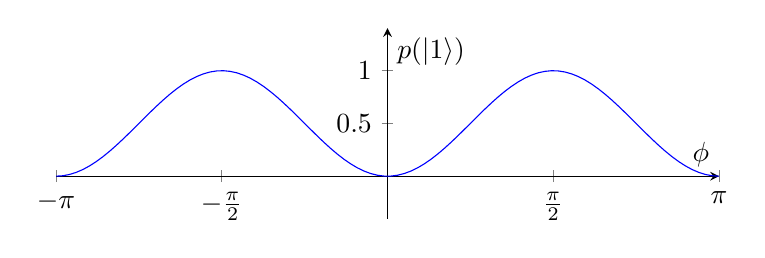
\begin{tikzpicture}
			\begin{axis}[
					axis lines = middle,
					xlabel = $\phi$,
					ylabel = {$p(\ket{1}$)},
					ymin = 0,
					ymax = 1,
					xtick={-pi, -pi/2, 0, pi/2, pi}, % Positions of the x-ticks
					xticklabels={$-\pi$, $-\frac{\pi}{2}$, $0$, $\frac{\pi}{2}$, $\pi$}, % Labels for the x-ticks
					width=10cm, % Width of the plot
					height=4cm, % Height of the plot
					axis equal, % Ensure x and y units are the same length
				]
				\addplot[
					domain=-pi:pi,
					samples=100,
					color=blue,
				]
				{sin(deg(x))^2};
			\end{axis}
		\end{tikzpicture}
	}
	\caption{probability of measuring $\ket{1}$ for each value of $\phi$}
	\label{interferencegraph}
\end{figure}
It is possible to observe in Figure \ref{interferencegraph}
that the output of the measure on the qubit depends only on the
ammout of fase shift that has been inflicted
to the qubit, this can be seen as a manifestation of the phenomenon
of interferece.

\newpage

\subsection{introduction to quantum universality}

The circuit used in the previous section allows to manipulate a qubit in
every possible way but it has to be noted that it utilizes a gate that
applyes an arbitrary ammount of phase shift.
Such gate has to be seen more like a family of gates.
It is interesting to know if it would be possible to achieve the same
result with a predeterminated and finite set of gates, that can actually
be built.
The short answer to this question is no, but we can get very close.
To elaborate more this answer we need to introduce a few definitions
regarding quantum universality.
\begin{itemize}

	\item
	      a \textbf{Strictly universal} set of gates can be used to equal
	      every possible gate


	\item
	      a \textbf{Prox universal} set of gate can approximate every possible gate to
	      arbitrary precision


\end{itemize}
Unfortunately there isn't and can't be a finite and strictly universal
set of ports because the space of unitary operators in a
Hilbert space is continuous while the possible circuits that can be built
from a finite set of them is just countable.\\
The proprety we can actually achieve in a real world circuit is
prox-universality.\\

\begin{theorem}
	The set of gates \{H, T\} is prox universal.
\end{theorem}
This result is due to the fact that the operators defined by HTHT and THTH
give rotations in two distint axis by an irrational multiple of $\pi$



\section{Many qubits systems}



\subsection{Many qubits gates}
It is possible to construct gates that involve many qubits combining their states.\\
The most common example of this kind of gates are controlled not gates.\\
A controlled not gate involves two qubits and has a control and a target qubit.\\
If the control qubit is in the state $\ket{1}$ the gate applies a bitflip
operator on the target qubit, otherwise it applies the identity.

%TODO talk about the imposiibility of quantum cloning

\newpage

\subsection{Quantum entanglement}

It often happens using many qubit gates that the states of the output
qubits are no longer independent from each other so the probability
of measuring a possible result on one qubit depends on the states of
other qubits involved in the transformation.
In this case we called this "bonded" qubits entangled.
a clear example of this can be found in the circuit in Figure \ref{entanglement}.\\

\begin{figure}[H]
	\centering
	\scalebox{1.5}{
		\begin{quantikz}
			\lstick{$\ket{0}$}\slice[style=blue, label style={pos=1, anchor=north}]{${\scriptstyle\ket{\psi_{t0}}}$}	& \gate{H}
			\slice[style=blue, label style={pos=1, anchor=north}]{${\scriptstyle\ket{\psi_{t1}}}$}	 &\ctrl{1}&\\
			\lstick{$\ket{0}$}&& \targ{} \slice[style=blue, label style={pos=1, anchor=north}]{${\scriptstyle\ket{\psi_{t2}}}$}	&
		\end{quantikz}
	}
	\caption{Bell state generator}
	\label{entanglement}
\end{figure}

\begin{itemize}
	\item $\ket{\psi_{t0}} = \ket{0} \otimes \ket{0}$
	\item $\ket{\psi_{t1}} = \dfrac{\ket{0}+\ket{1}}{\sqrt{2}} \otimes \ket{0} = \dfrac{\ket{00}+\ket{10}}{\sqrt{2}}$
	\item $\ket{\psi_{t2}} = \dfrac{\ket{00}+\ket{11}}{\sqrt{2}}$

\end{itemize}
It can be observed that the final state of the circuit can't be split
in a tensor product of states so it is possible to assign a state to
the system as a whole but not to the the individual qubits that compose it.
Moreover it is one of the four Bell states.
Such states have the interesting proprety of constituting a base for all
the states of two qubits.


\subsection{Universality for multiple qubits}
Knowing it is possible to make a circuit that arbitrarly approximates
every
single quantum gate what we could be interested in discovering is how
big that circuit would be.\\
That is known thanks to an amazing result by Solovay and Kitaev which
states
that the number of ports we need to aproximate a circuit with a certain
precision grows logaritmically with the precision we want to achieve.

\begin{theorem}[Solovay-Kitaev 1995]

	Given a strictly universal set of gates S which is closed under inversion,
	the number of gates needed to approximate every n qubit circuit made
	from S whith precision $\epsilon$ is
	$O\Bigl(n2^n+2^n\log_2 \Bigl( \dfrac{1}{\epsilon}\Bigl)\Bigl)$

\end{theorem}



\section{Representing uncertainty}

\subsection{Errors generate uncertainty}

To model an open quantum system we need to consider the fact that
our qubits will entangle with other quantum systems that we cannot control.
This will introduce some uncertanty both in the state of our quantum
system in each given time and the transformations that state will go trough.
The concepts of density operators and quantum operations will be presented to
model a partially unknown states and transformations.


\subsection{Uncertainty in quantum states}

To analyze a real world quantum system it is foundamental to consider
it a subsystem of a bigger system composed by our circuit and the
surrounding environment.

\subsubsection{Ensembles of states}

Let's suppose a qubit is prepared either in state $\ket{0}$ or in
state $\ket{1}$ based on the result of a coin toss.
In this case it is not possible to assign a state to such qubit
but it can be expected to get either result with probability
$\dfrac{1}{2}$  when we measure it.
This example can be generalized to when we have a so called
"ensemble of states" $\{p_i,\ket{\psi_i}\}$ which is a set of
states our system could be in each with an associate probability $p_i$
of the system actually being in that state.\\
This case suggest us that sometimes it is convenient to
shift our attention from the state of our system itself to the
statistical predictions we can make about the outcome of a measure on it.
Such can be achieved thanks to the density operator that
is usually identified with the letter $\rho$ and in the case of the above
mentioned ensamble would assume the form $\sum_i p_i \ket{\psi_i}\bra{\psi_i}$
which is the sum of the projectors on the states $\psi_i$ weighted with
probabilities $p_i$. \\
In the case when the ensemble is made by just one state,
that is when the state of our qubit is certain,
the density operator of our qubit is just the projector on
that state.
The outcome of a measure on a qubit is given by calculating
the trace of the operator given by the multiplication of our
measuring operator by the density operator.


\subsubsection{From system to subsystem}

When we study a quantum system we are not always interested in the
system as a whole, sometimes we care only about a fraction of it.
Compartmentalizing the system if for sure easy and intuitive when it
is in a pure state, but can be more intricate when we are talking about
an entangled state.\\
In this latter case in fact we are not able to assign a state to the
subsystem that is independent from the rest of the original system
and we have to rely on the possibility of making statistical
predictions about the outcomes of a measure on that subsystem.\\
This should suggest us that the density operator can come useful
again but the question remains how get the density operator that
describes a subsystem given the density operator of the system.
It turns out that the only way to obtain it is doing the partial
trace of the density operator of the all system.
This comes from the fact that we want to maintain consistency between
applying the same transformation to the whole system or to the
subsystem taken into consideration.
%TODO consider adding more details.

\subsubsection{The Bloch ball}


\subsection{Uncertainty in quantum transformations}

\subsubsection{System environment interaction}

It is often the case that the quantum system is embedded in an environment
that can't be control therefore it is important to consider the interaction
between the system and such environment.
Suppose the system starts in an initial state $\rho$ and the environment
starts in state $\rho_{env}$,
a unitary operator $U$ is
applied to them;
A the end the system will be in state

\begin{equation}
	\rho' = tr_{env} \left[U (\rho \otimes \rho_{env})U^\dag \right].
\end{equation}
The finel state $\rho'$ is often referred as $\mathcal {E}(\rho)$ and
$\mathcal {E}$ is said to be a quantum operation acting on the state $\rho$.

\subsubsection{The Operator sum representation}

It is useful to develop a self contained way to describe the evolution
of a system that takes into consideration only the part we have control of.
This is done by assuming the environment to always start in a pure state.
Such assumption is fair because it is always possible to choose the environment
"big enough" not to be entangled with any other state thanks to a procedure
called purification.
The traslation of the assumption on the above equation produces:
\begin{equation}
	\mathcal{E}(\rho) =  \sum_{k} \bra{e_k}U \left[ \rho \otimes \ket{e_0}\bra{e_0}
		\right] U^\dagger \ket{e_k} = \sum_k E_k \rho E_k^\dagger  \\
\end{equation}
where $E_k=\ket{e_k}U\ket{e_0}$ and the operation elements $E_k$ satisfy
the completness relation so $\sum_k E_k^\dagger E_k = I$
If $d$ is the dimension of the hilbert space whoose state is described by
$\rho$ it is always possible to describe every admissible quantum operation
with at most $d^2$ terms being the space of $d \times d $ matrices $d^2$-dimensional
vector space.

\subsubsection{Unitary freedom in the operator sum representation}

\begin{theorem}
	\label{freedom}
	Given the operations $\mathcal{E}$ and $\mathcal{F}$ with operation elements
	$\{E_1,...,E_m\}$ and $\{F_1,...,F_n\}$, after appending zero operators
	to the end of the shorter list to ensure that m=n,
	$\mathcal{E}=\mathcal{F}$ if and only if there exists an m by m unitary matrix
	of complex numbers $u_{ij}$ such that $E_i = \sum_j u_{ij} F_j$

\end{theorem}



\subsubsection{Common quantum channels}

Here is a list of the most common models of quantum channels and their respectiove
operator-sum representations:

\begin{itemize}

	\item the \textbf{Bit flip channel} can flip the state of a qubit applying
	      the operator $X$ with probability $1-p$ and do nothing with
	      probability $p$.
	      its operation elements are:
	      \begin{equation}
		      E_0 = \sqrt{p}I, \hspace{20pt} E_1 = \sqrt{1-p}X
	      \end{equation}

	\item the \textbf{Phase flip channel} can shift the phase by $\pi$ of a qubit applying
	      the operator $Z$ with probability $1-p$ and do nothing with
	      probability $p$.
	      its operation elements are:
	      \begin{equation}
		      E_0 = \sqrt{p}I, \hspace{20pt} E_1 = \sqrt{1-p}Z
	      \end{equation}

	\item the \textbf{Depolarizing channel} can substitute the state of the system with the
	      totally mixed state with probability $1-p$ and do nothing with
	      probability $p$.
	      The totally mixed state is a state with density operator $I/2$

	      that holds no information.
	      the operation elements of the depolarizing channel are:
	      \begin{equation}
		      E_0 = \sqrt{1-\tfrac{3}{4}p}I, \hspace{5pt} E_1 = \sqrt{1-p}X , \hspace{5pt}
		      E_2 = \sqrt{1-p}Y , \hspace{5pt} E_3 = \sqrt{1-p}Z
	      \end{equation}


\end{itemize}

\section{Measuring errors}

\subsection{The importance of distance measures}

When a system gets entangled with the environment the latter causes the system
to deviate from it's expected evolution giving birth to an error.
Considering only the presence or absence of errors though would be of little
information because errors can vary wildly based on how much they shift the
quantum state and so the probability of getting a certain result during
the measurement procedure.
The need for a way to measure the distance between two states to see, for example,
how much errors have shifted the system away from the desires state, has resolved
in the development of static distance measures.
Static distance measures are then used to derive ways to quantify how much quantum
information gets lost by a system during transformations which are dynamic distance
measures.


\subsection{Static distance measures}


The most common static distance measure for quantum states is the fidelity.
It derives from the classical fidelity which is a distance measure between
probability distributions.
The quantum fidelity of states $\rho$ and $\sigma$ is defined as:
\begin{equation}
	F(\rho,\sigma):=tr \sqrt{\rho^\frac{1}{2}\sigma\rho^\frac{1}{2}}
	\label{qfidelity}
\end{equation}
and when the operators $\rho$ and $\sigma$ commute they can be written as:

\begin {equation}
\rho = \sum_{i} r_i\ket{i}\bra{i}; \hspace{10pt} \sigma = \sum_{i} s_i \ket{i}\bra{i}
\end {equation}
so the equation \ref{qfidelity} becomes:

\begin{equation}
	F(\rho,\sigma) = tr \sqrt{\sum_{i} r_i s_i \ket{i}\bra{i} } = tr \left( \sum_{i} \sqrt{r_i s_i} \ket{i}\bra{i}
	\right) = \sum_{i}\sqrt{r_i s_i}
\end{equation}
where the last expression is exactly the classical fidelity between the eigenvalue
distributions $r_i$ and $s_i$ of $\rho$ and $\sigma$

the fidelity has some important proprieties:
\begin{itemize}
	\item Invariance under unitary transforms
	\item \textbf{Strong concavity}: let $p_i$ and $q_i$ be probability distributions
	      and $\rho_i$
	\item Monotonicity
	      %FIXME deshittify
\end{itemize}
\subsection{Dynamic distance measures}

It is also possible to use the fidelity to construct a way to to measure how
well quantum information is preserved during a generic quantum operation.
To do it what is usually evaluated is how a quantum operation preserves
entanglement.
This gives rise to the concept of entanglement fidelity which is a function
of the density operator of a state $\rho$ and a trace preserving quantum operation
$\mathcal{E}$.

\begin{equation}
	F(\rho,\mathcal{E}) := F(RQ,R'Q')^2 = \bra{RQ} \left[ (I_R \otimes \mathbb{E})(\ket{RQ}\bra{RQ}) \right] \ket{RQ}
\end{equation}



\section{Correcting errors}

\subsection{Brief introduction to classical error correction}

Correcting errors is an ancient problem that puzzled the minds of
information theorists long before the invention of quantum computation.
To achieve such task it is common to encode information in a subspace of
the space of messages that can be sent trough the channel to be able to
detect if a message has shifted away from this subspace because of an
error and, if possible, correct it.\\
A natural way of doing the above is using linear codes because they
enable a compact representation of the code itself.\\
A simple example of this concept is given by the three bit repetition
code.\\
To encode a message in this simple code we have to repeat each letter
or digit three times es: example $\rightarrow$ eeexxxaaammmpppllleee.\\
To decode a possible message we will choose from each triple the
letter that appears in the most occurrences es peexxxaanmmmpppllleee $\rightarrow$ example. \\
If the channel introduces few errors we will often be able to recover
the initial message completely.
The problem with this simple code lies in the fact that it is not very
efficient in terms of space occupied by the encoded message.
Further developments of this idea brought us codes like the Hamming
codes and the Reed-Solomon codes which are widely used to this day.


\subsection{Quantum coding theory}

\subsubsection{differences with the classical case}

Unfortunately when it comes to error correction quantum systems encounter
some additional problems unknown to classical systems and this makes the
procedure more complex.
\begin {itemize}

\item The \textbf{No cloning principle} shows that is impossible to generate
multiple copies of an unknown quantum state so the technique used for example
in classical repetition code is unfeasible without some adaptations.

\item Quantum states are by nature \textbf{continuous} as opposed to the
discrete states of a classical computer.
This makes so that errors that can occur are continuous too.

\item The measurement procedure on quantum states is \textbf{disruptive} so it is not
possible to know the state of a qubit in order to select the best procedure
to correct eventual errors on it.
\end{itemize}


Such problems have been tackled in the following ways.

\subsubsection{Entranglement instead of cloning}

The cloning done in classical error correction is substituted with
the creation of a group of entangled qubits which are called physical qubits
and encode the information of a single qubit, called logical qubit,  in order
to preserve it trough the noisy channel.


\subsubsection{Syndrome measurements}

The measurement is aimed at extracting the error syndrome which
is a quantity that contains information only about the error occurred
in the channel and not about the state of the system.
Not extracting any information from the state of the system
this measurement procedure avoids altering it.



\subsubsection{Finite error syndromes}

The solution presented in the previous paragraph would be impossible to
apply if the error syndromes would be infinite as it would be natural to
imagine.
Fortunately it is not the case but to understand the reason for such
an unexpected result it is necessary to introduce an intermediary step.

\begin{theorem}[Knill-Laflamme condition 1997]
	\label{conditions}
	Let $C$ be a quantum code and $P$ be the projector onto $C$.
	Suppose $\mathcal{E}$ is a quantum operation with operation elements $\{E_i\}$.
	A necessary and sufficient condition for the existence of an error-correction
	operation $\mathcal{R}$ correcting $\mathcal{E}$ on $C$ is that

	\begin{equation}
		P E_i^\dagger E_j P = \alpha_{ij} P
		\label{eccondition}
	\end{equation}
	for some Hermitian matrix $\alpha = (\alpha_{ij})$ of complex numbers.
\end{theorem}


\noindent $Proof$ \hspace{10pt}
The condition \ref{eccondition} is sufficient because it
is possible to explicitly construct an error-correction operation
$\mathcal{R}$ whenever it is satisfied.
To construct $\mathcal{R}$ a set of quantum error correction is picked
according to the condition \ref{eccondition}.
By assumption $\alpha$ is a Hermitian matrix, so it can be diagonalized
$d =u^\dagger \alpha u$ where u is an unitary matrix and d is diagonal.
Then the operators $F_k$ are defined in the following way:
\begin{equation}
	F_k := \sum_i u_{ik} E_i.
\end{equation}
Theorem \ref{freedom} shows that $\{F_k\}$ is also a set of operation
elements for $\mathcal{E}$ so it is possible to write:

\begin{equation}
	\label{condition2}
	P F_k^\dagger F_l P = \sum_{ij} u_{ki}^\dagger u_{jl} P E_{i}^\dagger E_j P.
\end{equation}
cobining \ref{condition2} with \ref{eccondition}
the condition becomes:

\begin{equation}
	P F_k^\dagger F_l P = \sum_{ij} u_{ki}^\dagger \alpha_{ij} u_{jl} P
\end{equation}
and since $d = u^\dagger \alpha u$

\begin{equation}
	\label{simplecondition}
	P F_k^\dagger F_l P = d_{kl}P
\end{equation}
which can be thought of as a simplification of the condition \ref{eccondition} ,
because $d_{kl}$ is diagonal.
Using the polar decomposition and the the equation \ref{simplecondition} it is
possible to see that for some unitary operator $U_k$

\begin{equation}
	F_k P = U_k \sqrt{PF_k^\dagger F_k P} = \sqrt{d_{kk}} U_k P
\end{equation}
The effect of $F_k$ is to rotate the coding subspace into a second subspace defined by
the projector $P_k$ which is defined in the following way:

\begin{equation}
	\label{defpk}
	P_k := U_k P U_k^\dagger = \dfrac{F_k P U_k^\dagger}{\sqrt{d_{kk}}}
\end{equation}
These subspaces are necessarily orthogonal because for equation \ref{simplecondition}
when $k \neq l$:

\begin{equation}
	P_l P_k = P_l^\dagger P_k = \dfrac{U_l P F_l^\dagger F_k P U_k^\dagger}{\sqrt{d_{ll}d_{kk}}} = 0
\end{equation}

\noindent In this construction the syndrome measurement is a projective measurement defined by
the operators $P_k$, augmented by an additional projector if necessary to satisfy
the completeness relation $\sum_k P_k = I$.
Recovery is accomplished simply by applying $U_k^\dagger$.
It is possible to verify that the error correction is appropriate calculating
$ \mathcal{R}(\mathcal{E}(\rho)) $ where $\mathcal{E}(\sigma) = U_k^\dagger P_k \sigma P_k U_k$
is the combined detection-recovery step.

\noindent Applying the definition \ref{defpk} and the condition \ref{simplecondition}
it is possible to derive that:

\begin{equation}
	U_k^\dagger P_k F_l \sqrt{\rho} = U_k^\dagger P_k^\dagger F_l P \sqrt{\rho}
\end{equation}

\begin{equation}
	=	\dfrac{U_k^\dagger U_k P F_k^\dagger F_l P \sqrt{\rho}}{\sqrt{d_{kk}}} = \dfrac{P F_k^\dagger F_l P \sqrt{\rho}}{\sqrt{d_{kk}}}
\end{equation}

\begin{equation}
	\label{conditionauxilary}
	= \delta_{kl} \sqrt{d_{kk}} P \sqrt{\rho} = \delta_{kl} \sqrt{d_{kk}} \sqrt{\rho}
\end{equation}
Thus:

\begin{equation}
	\mathcal{R}(\mathcal{E}(\rho)) = \sum_{kl} U_k^\dagger P_k F_l \rho F_l^\dagger P_k U_k = \sum_{kl} \delta_{kl} d_{kk} \rho \propto \rho
\end{equation}
as required.
\vspace{20pt}
To prove necessity suppose $\{E_i\}$ is a set of errors corrected by the error-correction
operation $\mathcal{R}$ with operation elements $\{R_j\}$.\\
Define a quantum operation $\mathcal{E}_C$ by $\mathcal{E}_C(\rho) := \mathcal{E}(P \rho P)$
Since $P \rho P$ is in the code space for all $\rho$, it follows that

\begin{equation}
	\mathcal{R}(\mathcal{E}(\rho)) \propto P \rho P
\end{equation}

\noindent for all states $\rho$. Moreover, the proportionality factor must be a constant c, not
depending on the imput state $\rho$, if both right and left side have to be linear.
Rewriting the last equation explicitly in terms of the operation elements gives

\begin{equation}
	\sum_{ij} R_j E_i P \rho P E_i^\dagger R_j^\dagger = cP \rho P
\end{equation}

\noindent This equation holds for all $\rho$. It follows that the quantum operation with operation
elements $\{R_jE_i\}$ is identical to the quantum operation with a single operation element
$\sqrt{c}P$. Theorem \ref{freedom} implies that there exist complex numbers
$c_{ki}$ such that
\begin{equation}
	R_k E_i P = c_{ki} P.
\end{equation}
Taking the adjoint of this equation gives $P E_i^\dagger R_k^\dagger = c_{ki}^* P$ and therefore\\
$P E_i^\dagger R_k^\dagger R_k E_j P =
	c_{ki}^* c_{kj} P$.
But $R$ is a trace-preserving operation,\\
so $\sum_k R_k^\dagger R_k = I$. \\ Summing the equation $P E_i^\dagger R_k^\dagger R_k E_j P = c_{ki}^* c_{kj} P$
over $k$ we deduce that:
\begin{equation}
	P E_i^\dagger E_j P = \alpha_{ij} P
\end{equation}
where $\alpha_{ij} \equiv \sum_k c_{ki}^* c_{kj}$ is just a Hermitian matrix of complex numbers.\\
These are the quantum error-correction conditions.


\begin{theorem}
	Suppose $C$ is a quantum code and $\mathcal{R}$ is the error-correction operation
	constructed in the proof of theorem \ref{conditions}to correct a
	noise process $\mathcal{E}$ with operation elements $\{E_i\}$.
	Suppose $\mathcal{F}$ is a quantum operation with operation elements $\{F_j\}$
	that can be written in the form $F_j = \sum_i m_{ij} E_i$ for some matrix $m_{ij}$
	of complex numbers.
	Then the error correction operation $\mathcal{R}$ also corrects for the effects
	of the noise process $\mathcal{F}$ on the code $C$
\end{theorem}


\noindent $Proof$
By Theorem \ref{conditions} the operaton elements
$\{E_i\}$ mustsatisfy the quantum eroor-correction condition $PE_iE_j^\dag P = \alpha_{ij}P$.
As shown in the proof of theorem \ref{conditions},
whithout loss of generality we may assume that the operation elements for $\mathcal{E}$
have been chosen such that $\alpha_{ij} = d_{ij}$ is diagonal with real entries.
The error-correction operation $\mathcal{R}$ has operation elements $U_k^\dagger P_k$, where by equation
\ref{conditionauxilary} the $U_k$ and $P_k$ are chosen such that for any $\rho$ in
the code space:

\begin{equation}
	U_k^\dagger P_k E_i \sqrt{\rho} = \delta_{ki} d_{kk} \sqrt{\rho}.
\end{equation}
Substituting $F_j = \sum_i m_{ji} E_i$ gives:
\begin{equation}
	U_k^\dagger P_k F_j \sqrt{\rho} = \sum_i m_{ji} \delta_{ki} d_{kk} \sqrt{\rho} = m_{jk} d_{kk} \sqrt{\rho},
\end{equation}
and thus
\begin{equation}
	R(F(\rho)) = \sum_{kj} U_k^\dagger P_k F_j \rho F_j^\dagger P_k U_k = \sum_{kj} |m_{jk}|^2 d_{kk} \rho \propto \rho,
\end{equation}
as required.


\subsection{Some examples of quantum codes}

\subsubsection{Quantum repetition codes}

Quantum repetition codes are similar to classical ones with the difference that, for the
above mentioned reasons, they use entanglement instead of cloning.
Simple repetition codes cannot correct an arbitrary error on a single qubit but they can
be constructed to correct errors on a given quantum channel.
Some examples are

\subsubsection{The Shor code}

\subsubsection{Degenerate codes}

\subsubsection{CSS codes}

\subsubsection{Stabilizer codes}




\end{document}
